\documentclass[11pt,letterpaper]{article}
\usepackage[lmargin=1in,rmargin=1in,tmargin=1in,bmargin=1in]{geometry}
\usepackage{../style/homework}
\usepackage{../style/commands}
\setbool{quotetype}{true} % True: Side; False: Under
\setbool{hideans}{true} % Student: True; Instructor: False

% -------------------
% Content
% -------------------
\begin{document}

\homework{9: Due 04/14}{Poetry is as precise a thing as geometry.}{Gustave Flaubert}

% Problem 1
\problem{10} Showing all your work, complete the following:
	\begin{enumerate}[(a)]
	\item Find the interior and exterior angles for a regular polygon with 22 sides. 
	\item Find the smallest angle between the hour and minute hand of an analog clock at 10:20. 
	\item Find $x$ in the diagram below:
		\[
		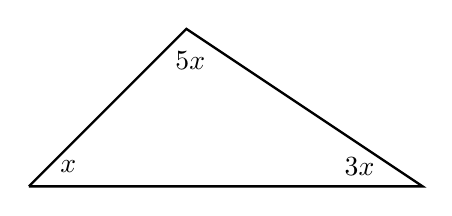
\begin{tikzpicture}
		\draw[line width=0.03cm] (0,0) -- (2,2) -- (5,0) -- (0,0);
		\node at (0.5,0.25) {$x$};
		\node at (2.05,1.6) {$5x$};
		\node at (4.2,0.25) {$3x$};
		\end{tikzpicture}
		\]
	\end{enumerate}



\newpage



% Problem 2
\problem{10} Assuming that the two horizontal lines are parallel, find all the angles labeled in the diagram below:
	\[
	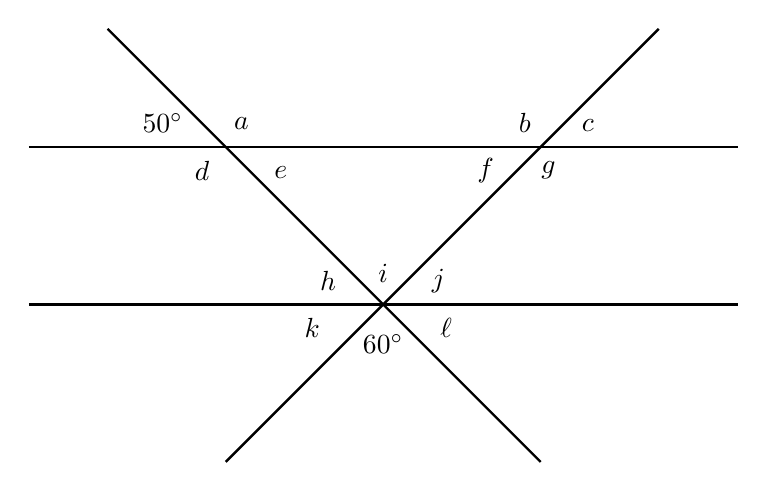
\begin{tikzpicture}
	\draw[line width=0.03cm] (-4.5,2) -- (4.5,2);
	\draw[line width=0.03cm] (-4.5,0) -- (4.5,0);
	\draw[line width=0.03cm] (-2,-2) -- (3.5,3.5);
	\draw[line width=0.03cm] (-3.5,3.5) -- (2,-2);
	\node at (-2.8,2.3) {$50^\circ$};
	\node at (-1.8,2.3) {$a$};
	\node at (1.8,2.3) {$b$};
	\node at (2.6,2.27) {$c$};
	\node at (-2.3,1.7) {$d$};
	\node at (-1.3,1.67) {$e$};
	\node at (1.3,1.7) {$f$};
	\node at (2.1,1.7) {$g$};
	\node at (-0.7,0.3) {$h$};
	\node at (0,0.4) {$i$};
	\node at (0.7,0.3) {$j$};
	\node at (-0.9,-0.3) {$k$};
	\node at (0,-0.5) {$60^\circ$};
	\node at (0.8,-0.3) {$\ell$};
	\end{tikzpicture}
	\]



\newpage



% Problem 3
\problem{10} A student claims that all rectangles are always squares, rhombuses are never squares, and trapezoids are sometimes squares. Which, if any, of these statements are correct and which are incorrect? How would you help this student understand these concepts? 


\end{document}